\chapter{Finite Differences} \label{ch:finitediff}

\epigraph{``Our goal should be to understand our differences.''}
{{\normalfont ---\ James D. Watson}}

\section{Introduction}
Most geophysical fields are governed by partial differential equations that express conservation of mass, energy, or momentum. In earlier chapters, we developed these equations analytically and explored their physical meaning through idealized geometries and closed-form solutions. Those analytic solutions are indispensable for building intuition, but they are also limited. Real geologic systems rarely conform to simple geometries, constant material properties, or uniform boundary conditions. At some point, the Earth becomes too complicated to solve with pencil and paper.

\textbf{Finite difference methods} provide a bridge between the governing equations of geophysics and the complexity of real Earth systems. Rather than attempting to solve a partial differential equation everywhere at once, we approximate it by enforcing its local balance on a discrete grid in space and time. In doing so, we \emph{replace continuous derivatives with differences between neighboring points}, turning differential equations into algebraic ones that can be solved on a computer.

Although finite difference methods are often introduced as numerical tools, their deeper significance is physical rather than computational. Each finite difference approximation represents a local statement of conservation. For example, the second spatial derivative in a diffusion equation measures local curvature of a field; in discrete form, it compares the value at one point to the average of its neighbors. Diffusion, whether of heat, chemical species, or electric current, becomes a process of local balancing repeated across the domain.

Throughout this chapter we use temperature as a unifying example, drawing on geothermics to illustrate both steady-state and time-dependent behavior. This choice is not restrictive. The same finite difference formulations apply to gravitational and electric potentials, chemical concentration, groundwater head, and displacement fields. Temperature provides a familiar and physically intuitive context in which gradients, curvature, boundary conditions, and time dependence can be understood concretely.

A central theme of this chapter is that the behavior of finite difference solutions depends fundamentally on the type of partial differential equation being solved. Elliptic equations, such as Poisson's and Laplace's equations for steady-state heat conduction or gravity, lead to systems of algebraic equations that enforce instantaneous balance throughout the domain. Parabolic equations, such as the heat diffusion equation, introduce storage and time dependence, requiring solutions to be advanced incrementally in time and giving rise to stability constraints and characteristic diffusion timescales. Hyperbolic equations, which govern wave propagation, impose entirely different numerical constraints related to causality and finite propagation speed.

Understanding these distinctions is essential. Finite difference methods do not merely approximate derivatives; they encode the physics of how information, energy, or mass moves through the Earth. Choices about grid spacing, time step, and boundary conditions are therefore not purely numerical decisions. They reflect assumptions about scales, processes, and the physical regime in which a model is valid.

This chapter introduces finite difference methods with three goals. First, to show how spatial and temporal derivatives are approximated in a way that respects the underlying conservation laws. Second, to connect numerical behavior directly to the elliptic, parabolic, and hyperbolic nature of geophysical equations. Third, to provide a foundation for forward modeling and inversion in later chapters, where numerical solutions become unavoidable.

By the end of this chapter, finite differences should no longer appear as a black-box numerical technique, but as a natural and physically transparent extension of the governing equations that underlie all of geophysics. Whether or not you pursue a career in geophysics, finite difference methods are widely used across science and engineering wherever spatial and temporal processes are governed by partial differential equations.

\subsection{Lithospheric Temperatures: A Unifying Example}

Before introducing the mechanics of finite difference approximations, it is useful to anchor the discussion in equations that are already familiar.  Throughout earlier chapters, we encountered a small number of governing equations that recur across geophysics, differing not in form but in physical fields and properties.

Here we return to those equations using temperature as a unifying example.  Our goal is not to derive them again, but to show how the same mathematical structure leads to very different numerical behavior once the equations are discretized in space and time.

Let the temperature field be
\[
T = T(\vb{x},t),
\]
governed by one of the following PDEs:

\begin{itemize}
  \item \textbf{Elliptic (steady state heat conduction):}
  \[
  \nabla^2 T = -\frac{A}{k},
  \]
  where $A$ is internal heat production and $k$ is thermal conductivity.

  \item \textbf{Parabolic (heat diffusion):}
  \[
  \frac{\partial T}{\partial t} = \kappa \nabla^2 T,
  \]
  where $\kappa = k/(\rho c_p)$ is thermal diffusivity.

  \item \textbf{Hyperbolic (waves, later chapters):}
  \[
  \frac{\partial^2 T}{\partial t^2} = c^2 \nabla^2 T.
  \]
\end{itemize}

The finite difference methods developed here are identical in spirit for all three cases; what differs is how information propagates through the domain.

Before discretizing these equations, it is useful to visualize the physical system they describe Figure~\ref{fig:xseciton}.

\begin{figure}
    \centering
    %\includegraphics[]{numerical/figures/.eps}
    \caption{A geologic cross-section of ???.  The model suggests smoothly varying layer interfaces with the occasional step from a fault. Each rock unit is assumed homogenous with a unique set of physical properties that describes it. This model will form the basis for developing the discrete grid for finite difference modelling.}
    \label{ref:xsection}
\end{figure}


\section{From Continuous Derivatives to Discrete Differences}

\subsection{Taylor Series Expansion: Local Approximation}

Finite difference methods rely on a simple but powerful mathematical idea: a smooth function can be represented locally by a polynomial whose coefficients are determined by its derivatives at a point.  Finite difference approximations are built on Taylor series expansions.  Although Taylor series are often introduced in mathematics courses, many students may not have seen them recently, so we briefly summarize their role here.

A Taylor series provides a local representation of a function in the neighborhood of a point. It expresses the value of a function at nearby locations in terms of its value and derivatives evaluated at a single point.  In essence, a Taylor series answers the question: if we know how a function behaves at one location, how well can we predict its behavior a short distance away?

Taylor series are especially useful in numerical methods because they provide a systematic way to relate derivatives to differences between values at nearby points. Truncating a Taylor series after a finite number of terms produces an approximation whose accuracy depends on the spacing between points. This truncation is the origin of discretization error in finite difference methods.

Let $f(x)$ be a sufficiently smooth scalar field. The Taylor series expansion
of $f$ about the point $x_i$ expresses the value of the function nearby as
\[
f(x_i + \Delta x)
=
f(x_i)
+ \Delta x \eval{\dv{f}{x}}_{x=x_i}
+ \frac{\Delta x^2}{2!} \eval{\dv[2]{f}{x}}_{x=x_i}
+ \frac{\Delta x^3}{3!} \eval{\dv[3]{f}{x}}_{x=x_i}
+ \cdots ,
\]
where $!$ indicates a factorial ($n! = \prod_{i=1}^n i$) and the ellipsis indicates higher-order derivative terms.

This expansion is not an approximation; it is an exact representation of the function provided all terms are retained. In practice, however, we truncate the series after a finite number of terms. Doing so converts the series into an approximation whose accuracy depends on both the spacing $\Delta x$ and the order at which the series is truncated.

Taylor series are useful because they allow derivatives to be related to differences between function values at nearby points. This makes them the natural mathematical foundation for finite difference methods, which replace continuous derivatives with discrete approximations on a grid.

In the discussion that follows, the function $f(x)$ represents a generic scalar field. For most of this chapter, we will use $T$ rather than $f$, but the same approximations apply equally to other geophysical fields such as gravitational potential, electric potential, chemical concentration, or displacement.

\subsection{Approximating derivatives}
\subsubsection{First-Order derivatives}

Finite difference approximations arise naturally from Taylor series
expansions. This connection is important because it makes explicit that
numerical derivatives are not exact, but controlled approximations with
well-defined error.

Consider a smooth function $f(x)$ expanded about the point $x_i$.  We can approximate the first derivative ($\eval{\dv{f}{x}}_{x=x_i}$) using the Taylor Series expansion as either a forward difference,
\begin{equation}
    f(x_i + \Delta x) \approx
    f(x_i)
    + \Delta x \eval{\dv{f}{x}}_{x_i}
    + \frac{\Delta x^2}{2!} \eval{\dv[2]{f}{x}}_{x_i}
    + \frac{\Delta x^3}{3!} \eval{\dv[3]{f}{x}}_{x_i}
    + \cdots,
    \label{eq:ftaylor}
\end{equation}
or a backward difference,
\begin{equation}
    f(x_i - \Delta x) \approx
    f(x_i)
    - \Delta x \eval{\dv{T}{x}}_{x_i}
    + \frac{\Delta x^2}{2!} \eval{\dv[2]{f}{x}}_{x_i}
    - \frac{\Delta x^3}{3!} \eval{\dv[3]{f}{x}}_{x_i}
    + \cdots.
    \label{eq:btaylor}
\end{equation}
Note the difference in signs between the two cases.

Truncation converts an exact representation into an approximation, and the omitted terms define the error introduced by the approximation. Retaining fewer terms leads to larger errors, while retaining more terms improves accuracy at the cost of additional complexity.  If we retain only the first derivative term in the forward expansion and neglect all higher-order terms, after rearranging to isolate for the derivative we obtain 
\begin{equation}
    \coreeq
    \text{Forward difference:}\quad
    \eval{\dv{f}{x}}_{x_i} \approx \frac{f(x_i + \Delta x) - f(x_i)}{\Delta x}.
    \label{eq:ffd}
\end{equation}
This forward difference approximation estimates the derivative at $x_i$ using information from the point ahead of it (Figure~\ref{fig:fddiscrete}). Because it is based on a one-sided expansion, the neglected higher-order terms introduce a systematic error.  Similarly, truncating the backward expansion after the first derivative term yields
\begin{equation}
    \coreeq
    \text{Backward difference:}\quad
    \eval{\dv{f}{x}}_{x_i} \approx \frac{f(x_i) - f(x_i - \Delta x)}{\Delta x}.
    \label{eq:bfd}
\end{equation}
This backward difference approximation uses information from the point behind $x_i$ (Figure~\ref{fig:fddiscrete}) and introduces a different truncation error of comparable magnitude.  Both forward and backward differences are first-order accurate, meaning that their leading error term scales linearly with the grid spacing $\Delta x$.
\begin{figure}[bth]
    \centering
    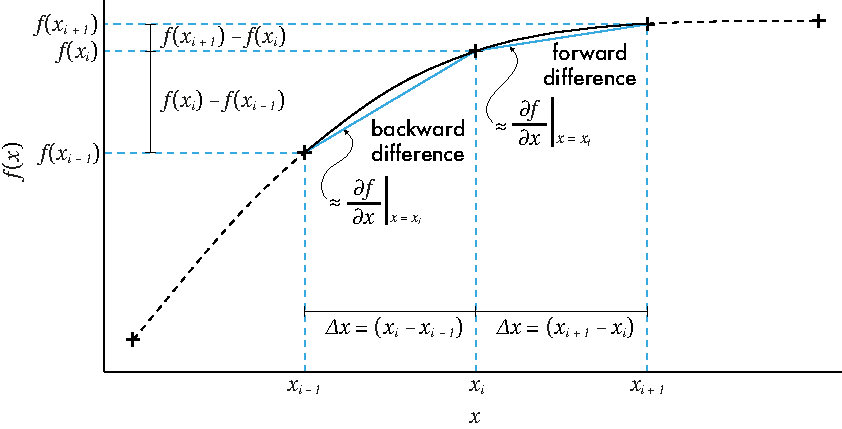
\includegraphics[]{numerical/figures/fddiscrete.pdf}
    \caption{Formulation of finite differences by discretizing a function.  The backward and forward differences are identified by the line segments between the nodes preceding and succeeding $z_i$, respectively.}
    \label{fig:fddiscrete}
\end{figure}

A more accurate approximation can be obtained by taking the arithmetic mean of the forward and backward differences. If we add the forward and backward Taylor expansions (Equations:~\ref{eq:ftaylor} and~\ref{eq:btaylor}) and divide by $2\Delta x$, the odd-order derivative terms cancel, yielding a symmetric approximation.  After solving for the derivative,
\begin{equation}
    \coreeq
    \text{Central difference}\quad
    \eval{\dv{f}{x}}_{x_i} \approx \frac{f(x_i + \Delta x) - f(x_i - \Delta x)}{2\Delta x}.
    \label{eq:cfd}
\end{equation}
This is known as the \emph{central difference} approximation. Because the leading-order asymmetric error terms cancel, the central difference is second-order accurate: its leading truncation error scales with $\Delta x^2$.  This cancellation illustrates two important principles in numerical methods:
\begin{itemize}
    \item symmetry improves accuracy---central differences use information from both sides of a point and therefore provide a better local approximation to the derivative than one-sided schemes; and
    \item finite difference methods do not eliminate error, they control it---the choice of grid spacing determines the magnitude of truncation error, while the choice of time step and scheme determines how that error propagates through a solution.
\end{itemize}

Central differences are preferred throughout most of a numerical domain. However, near boundaries, where information from one side of a node is unavailable, we are often forced to use forward or backward differences. The treatment of such boundary regions is discussed later when we consider discretized domains and boundary conditions.

\subsubsection{Second-Order Derivatives}

Many of the governing equations encountered in geophysics involve second-order spatial derivatives. To construct a finite difference approximation to the second derivative, we again begin with Taylor series expansions about the point $x_i$.

Add Equations~\ref{eq:ftaylor} and \ref{eq:btaylor} to combine the two expressions. As before, the odd-order derivative terms cancel, yielding
\[
    f(x_i + \Delta x) + f(x_i - \Delta x) =
    2 f(x_i) + \Delta x^2 \eval{\dv[2]{f}{x}}_{x_i} + \mathcal{O}(\Delta x^4).
\]

Rearranging to isolate the second derivative gives the central difference approximation
\[
    \coreeq
    \eval{\dv[2]{f}{x}}_{x_i} \approx
    \frac{f(x_i + \Delta x) - 2 f(x_i) + f(x_i - \Delta x)}{\Delta x^2}.
\]

This expression is second-order accurate: the leading truncation error scales with $\Delta x^2$. As with the first derivative, the improved accuracy arises from symmetry. By using information on both sides of the point $x_i$, the central difference eliminates the leading asymmetric error terms that would appear in one-sided approximations.

Second-order finite difference approximations of this form are fundamental to geophysical modeling. They appear directly in Poisson's equation, the diffusion equation, and the wave equation, and therefore play a central role in modeling potential fields, heat transport, and wave propagation.


\section{Discretizing Space}
In the previous section we focused on the mathematical theory to derive finite difference approximations to first- and second-order spatial derivatives using Taylor series.  Finite difference methods replace this continuous description with a discrete representation that samples the field at a finite number of locations. This step completes the transition from continuous governing equations to a numerical representation suitable for computation.

Using the cross section in Figure~\ref{fig:xsection} as a basis to construct a discrete grid (Figure~\ref{fig:xsection2}), the modeller must make some choices about row/column spacing.  The more nodes in the final mesh, the longer it will take to solve needs to balance the desired accuracy of the finite difference approximations, which improves as the number of nodes increase.  More nodes also makes the model more faithful to the smooth model geometry.

\begin{figure}
    \centering
    %\includegraphics[]{numerical/figures/.eps}
    \caption{A discritized geologic cross-section of ???.  Each rock unit is assumed homogenous with a unique set of physical properties that describes it. This model will be used for producing numerical models.}
    \label{ref:xsection2}
\end{figure}

Throughout this section we specialize to temperature, $T$, and adopt $z$ as the spatial coordinate, reflecting the vertical structure of the Earth that dominates many geothermic problems. This choice is one of physical convenience rather than mathematical necessity; the same discretization principles apply in any spatial direction and will later be extended to two-dimensional domains.

\subsection{Discretizing a one-dimensional domain}

Consider a one-dimensional vertical domain extending from the Earth's surface to some depth. We divide this domain into a finite set of discrete nodes located at depths $z_i$, where the spacing between adjacent nodes is $\Delta z$ (Figure~\ref{fig:znodes}). The temperature field is represented by its value at each node,
\[
T_j \equiv T(z_j).
\]
Between nodes, the temperature field is not explicitly represented. Instead, its behavior is inferred through finite difference operators that relate the temperature at each node to its neighbors. For one-dimensional problems, each node represents a depth at which temperature is evaluated.
\begin{figure}[bth]
    \centering
    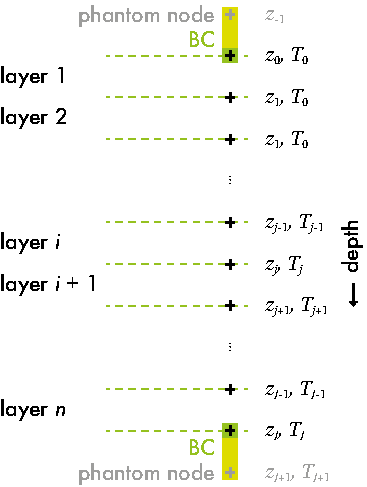
\includegraphics[]{numerical/figures/znodes.pdf}
    \caption{A one-dimensional discretization in space. Physical properties may
    be ascribed to the layers between each node (for one-dimension).  Phantom
    nodes may be placed outside the domain when flux boundary conditions are
    used.}
    \label{fig:znodes}
\end{figure}

Material properties may be associated either with the nodes themselves or with the intervals between nodes, depending on the formulation. For example, temperature is naturally defined at nodes, whereas properties such as thermal conductivity and heat production may be defined either at nodes or at the interfaces between them.

The choice of grid spacing $\Delta z$ is a modeling decision with direct physical consequences. Smaller values of $\Delta z$ reduce truncation error in finite difference approximations and allow sharper thermal gradients to be resolved. However, decreasing $\Delta z$ increases the number of nodes and therefore the computational cost of a solution.

In practice, grid spacing must balance accuracy against efficiency. A common approach is to repeat a calculation with progressively finer grids and verify that the solution converges within an acceptable tolerance. If halving $\Delta z$ produces negligible changes in the solution, the grid is sufficiently fine for the problem at hand.

Once the spatial domain has been discretized, the finite difference operators derived earlier are applied directly to the nodal values of temperature. For example, the second-order central difference approximation to the second derivative with respect to depth is written in discrete form as
\[
    \eval{\pdv[2]{T}{z}}_{z=z_j} \;\longrightarrow\;
    \frac{T_{j+1} - 2T_j + T_{j-1}}{\Delta z^2}.
\]

This operator measures the local curvature of the temperature field. If $T_j$ is larger than the average of its neighboring values, the curvature is negative and diffusion acts to reduce $T_j$. In this way, finite difference methods implement diffusion as a local balancing process repeated throughout the domain.

The pattern of nodes used to evaluate a finite difference operator is called a \emph{stencil}. For the second derivative in one dimension, the stencil consists of a central node and its immediate neighbors above and below (Figure~\ref{fig:fdstencils}). The stencil makes explicit that finite difference methods rely only on local information to approximate spatial derivatives.
\begin{figure}[htb]
    \centering
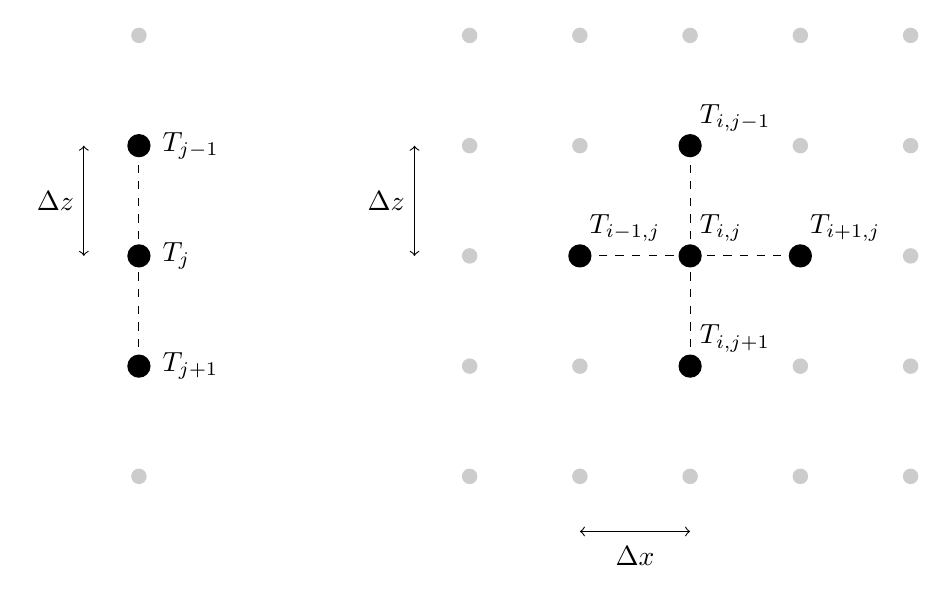
\begin{tikzpicture}[scale=1.4]
    \begin{scope}
        % Background grid nodes (faded)
        \foreach \k in {-2,2} {
            \fill[gray!40] (0,-\k) circle (2pt);
        }

        % Stencil nodes
        \fill (0,0) circle (3pt) node[right,xshift=5] {$T_{j}$};
        \fill (0,1) circle (3pt) node[right,xshift=5] {$T_{j-1}$};
        \fill (0,-1) circle (3pt) node[right,xshift=5] {$T_{j+1}$};

        % Dashed connections
        \draw[dashed] (0,0) -- (0,1);
        \draw[dashed] (0,0) -- (0,-1);

        % Delta z annotation
        \draw[<->] (-0.5,0) -- (-0.5,1) node[midway,left] {$\Delta z$};
    \end{scope}

    \begin{scope}[xshift=5cm]
        % Background grid (faded)
        \foreach \x in {-2,-1,0,1,2} {
            \foreach \z in {-2,-1,0,1,2} {
                \fill[gray!40] (\x,\z) circle (2pt);
            }
        }

        % Stencil nodes
        \fill (0,0) circle (3pt) node[right,yshift=10] {$T_{i,j}$};
        \fill (1,0) circle (3pt) node[right,yshift=10] {$T_{i+1,j}$};
        \fill (-1,0) circle (3pt) node[right,yshift=10] {$T_{i-1,j}$};
        \fill (0,1) circle (3pt) node[right,yshift=10] {$T_{i,j-1}$};
        \fill (0,-1) circle (3pt) node[right,yshift=10] {$T_{i,j+1}$};

        % Dashed stencil connections
        \draw[dashed] (0,0) -- (1,0);
        \draw[dashed] (0,0) -- (-1,0);
        \draw[dashed] (0,0) -- (0,1);
        \draw[dashed] (0,0) -- (0,-1);

        % Delta z annotation
        \draw[<->] (-2.5,0) -- (-2.5,1) node[midway,left] {$\Delta z$};
        \draw[<->] (-1,-2.5) -- (0,-2.5) node[midway,below,yshift=-2pt] {$\Delta x$};
    \end{scope}
\end{tikzpicture}
\caption{Stencils are the constructed connections between nodes used in finite difference approximations.  (a) One-dimensional finite difference stencil for the first and second derivative.  (b) Five-point stencil for the two-dimensional, first-derivative (gradient and divergence) or second-derivative (Laplacian).}
\label{fig:fdstencils}
\end{figure}

\subsection{Extension to two dimensions}

For problems involving lateral as well as vertical variations, the temperature field is written as $T(x,z,t)$. Discretizing both spatial directions leads to a two-dimensional grid with nodes indexed by $(i,j)$, where $i$ refers to the horizontal coordinate $x$ and $j$ to depth $z$.

Applying the same finite difference operators in each direction yields the standard five-point approximation to the Laplacian,
\[
    \eval{\pdv{T}{x}}_{x=x_i} + \eval{\pdv{T}{z}}_{z=zj} =  \;\longrightarrow\;
    \frac{T_{i+1,j} + T_{i-1,j} + T_{i,j+1} + T_{i,j-1} - 4T_{i,j}}{\Delta x^2},
\]
where $\Delta x = \Delta z$ is assumed for simplicity. This operator is the direct two-dimensional analogue of the one-dimensional second difference and follows from the same Taylor series arguments developed earlier.  The second difference measures the local \emph{curvature} of the temperature field. If $T_{i,j}$ is greater than the average of its neighbors, diffusion removes heat from that location. Finite differences therefore implement diffusion as a local balancing process.
The 2-D stencil in Figure~\ref{fig:fdstencils} can be used for either first- or second-order central differences.  

The discretization of space completes the transition from a continuous physical description of the Earth to a numerical representation suitable for computation. In the following sections we examine how boundary conditions are applied on this discrete grid and how time dependence is incorporated for transient problems.

\subsection{Steady-state problems: Poisson's equation}

The spatial discretization developed above can be used directly to solve
steady-state problems governed by elliptic equations. A common example in
geophysics is steady-state heat conduction with internal heat production,
described by Poisson's equation,
\[
    \pdv{}{z}\!\left(k \pdv{T}{z}\right) = -A,
\]
where $k$ is thermal conductivity and $A$ is volumetric heat production.

For constant thermal conductivity, this reduces to
\[
    \pdv[2]{T}{z} = -\frac{A}{k}.
\]
Using the second-order central difference derived earlier, the finite
difference approximation at node $z_j$ is
\[
    \frac{T_{j+1} - 2T_j + T_{j-1}}{\Delta z^2} = -\frac{A_j}{k}.
\]

Applying this equation at every interior node produces a system of linear
equations that can be written in matrix form,
\[
    \begin{bmatrix}
        1 & 0 & 0 & 0 & \cdots & 0 & 0 \\
        1 & -2 & 1 & 0 & \cdots & 0 & 0 \\
        0 & 1 & -2 & 1 & \cdots & 0 & 0 \\
        \vdots & \ddots & \ddots & \ddots & & \vdots & \vdots \\
        0 & \cdots & 0 & 1 & -2 & 1 & 0 \\
        0 & \cdots & 0 & 0 & 1 & -2 & 1 \\
        0 & 0 & 0 & 0 & 0 & 0 & 1
    \end{bmatrix}
    \begin{bmatrix}
        T_0 \\
        T_1 \\
        T_2 \\
        \vdots \\
        T_{J-2} \\
        T_{J-1} \\
        T_J
    \end{bmatrix}
    =
    \begin{bmatrix}
        T_0^{\text{bc}} \\
        -\dfrac{A_1 \Delta z^2}{k} \\
        -\dfrac{A_2 \Delta z^2}{k} \\
        \vdots \\
        -\dfrac{A_{J-2} \Delta z^2}{k} \\
        -\dfrac{A_{J-1} \Delta z^2}{k} \\
        T_J^{\text{bc}}
    \end{bmatrix}.
\]
Boundary conditions supply the additional equations needed to close the system. Solving this system yields the steady-state temperature profile directly, without time stepping.  This system is tridiagonal, reflecting the local nature of the finite difference stencil. If thermal conductivity varies with depth, the coefficients in the matrix change, but the tridiagonal structure of the system is preserved.

\subsection{Boundary Conditions}

Just as boundary conditions are required to obtain analytic solutions to partial differential equations, they are also essential for numerical solutions. In finite difference methods, boundary conditions provide the additional information needed to evaluate derivatives at the edges of a discretized domain and therefore play a central role in determining the
behavior of the solution.

Unlike interior points, where symmetric finite difference operators can be applied, boundary nodes lack information on one side. As a result, the choice and implementation of boundary conditions directly affect numerical accuracy and stability. In many practical problems, numerical errors are dominated not by the discretization of the interior, but by the treatment of boundaries.

\subsubsection{Boundary Condition Types}

Boundary conditions encountered in geophysical modeling are commonly grouped into three main types (Table~\ref{tab:bc}). A fourth category, sometimes referred to as a Cauchy condition, arises when different boundary types are applied on different parts of the domain.
\begin{table}[htbp]
    \centering
    \caption{Types of boundary conditions for discrete PDE methods.}
    \label{tab:bc}
    \begin{tabularx}{0.75\textwidth}{llX}
    \toprule
    Type & Mathematical form & Geophysical meaning \\
    \midrule
    Dirichlet (fixed) & $T = T_0$ & Fixed temperature (e.g., surface or magma temperature) \\
    Neumann (fixed flux) & $\displaystyle \pdv{T}{z} = \frac{q}{k}$ & Prescribed heat flux (e.g., basal heat flow) \\
    Neumann (zero flux) & $\displaystyle \pdv{T}{z} = 0$ & No heat flow across boundary (reflecting) \\
    Robin (mixed) & $aT + b\pdv{T}{z} = c$ & Coupled boundary (e.g., atmosphere--ground exchange) \\
    \bottomrule
    \end{tabularx}
\end{table}

A \emph{Dirichlet}, or fixed, boundary condition specifies the value of the field at the boundary and is straightforward to implement numerically.

A \emph{Neumann}, or fixed-flux, boundary condition specifies the gradient of the field at the boundary and therefore constrains the flow of heat rather than the temperature itself. A special case of the Neumann condition is the zero-flux boundary, which enforces no heat transfer across the boundary.

\emph{Robin} boundary conditions represent a linear combination of value and flux at the same boundary and commonly arise when the boundary interacts with an external reservoir, such as heat exchange between the ground and the atmosphere.

\emph{Cauchy} boundary conditions, in the strict mathematical sense, refer to situations where different boundary types are applied on different parts of the domain. In practice, most geophysical applications can be described using Dirichlet, Neumann, or Robin conditions.

In a finite difference model, boundary conditions must be enforced at specific
nodes. For Dirichlet conditions, this is accomplished by directly assigning
the boundary value to the appropriate node.

\subsection{Flux Conditions at Boundaries}

Neumann and Robin conditions require additional care because they involve derivatives at the boundary. Evaluating a derivative at a boundary node requires information beyond the edge of the computational domain. To handle this, it is common to introduce a \emph{phantom node} outside the domain.

For example, consider a Neumann boundary condition imposed at the surface,
\[
    \left.\pdv{T}{z}\right|_{z=z_0} = g.
\]
Using a finite difference approximation, this derivative can be written as
\[
    \frac{T(z_1) - T(z_{-1})}{2\Delta z} = g,
\]
where $T(z_{-1})$ is a phantom node located outside the domain. This relation allows the phantom-node value to be expressed in terms of interior nodes and the prescribed flux, ensuring that the boundary condition is satisfied while maintaining second-order accuracy.

Boundary conditions do more than close a mathematical system; they encode physical assumptions about how the modeled region interacts with its surroundings. This is especially important in geophysical problems dominated by vertical heat flow.

A fixed-flux boundary condition allows heat to enter or leave the domain at a specified rate. For example, prescribing basal heat flow permits heat to continuously enter the lithosphere from below. In contrast, a zero-flux boundary condition is reflecting: it prevents heat from crossing the boundary entirely. Any heat that would otherwise leave the system is instead reflected back into the domain.

When applied to vertical boundaries in models dominated by vertical heat transport, zero-flux conditions can strongly influence the solution. They effectively assume that no lateral heat exchange occurs across the boundary, which may or may not be physically appropriate depending on the scale of the model and the geological setting. As a result, zero-flux boundaries should be used deliberately and interpreted carefully.

\subsection{Why boundary conditions dominate solutions}

Because elliptic and parabolic equations communicate information throughout the domain, boundary conditions exert a global influence on the solution. An incorrect or poorly implemented boundary condition can overwhelm the effects of interior discretization, leading to solutions that are numerically stable but physically misleading.

For this reason, boundary conditions should be viewed not as technical details, but as integral components of the physical model. In geophysical applications, they encode assumptions about surface processes, basal heat input, and the degree to which the modeled system is isolated or interacting with its surroundings.

\subsection{Sharp property gradients}

Many geologic systems contain sharp spatial variations in material properties.  Examples include layered sediments, faults, lithologic contacts, and the transition from crust to mantle. In such cases, thermal conductivity, heat capacity, or diffusivity may change abruptly over distances comparable to or smaller than the grid spacing.

Sharp property gradients present a challenge for finite difference methods because standard central difference operators implicitly assume that coefficients vary smoothly across a stencil. When this assumption is violated, naïve discretizations can produce unphysical temperature profiles or incorrect heat fluxes.

For heat conduction, the physically relevant quantity is not temperature itself, but heat flux. At a material interface, temperature may have a kink (change in gradient), but heat flux must remain continuous. In one dimension, this requires
\[
    k_1 \eval{\pdv{T}{z}}_{\text{above}} = k_2 \eval{\pdv{T}{z}}_{\text{below}} .
\]

Finite difference schemes must therefore be constructed to preserve flux continuity across interfaces. Harmonic averaging and grid refinement are two methods that can be employed at abrupt boundaries.

A common and effective approach is to define thermal conductivity at the interfaces between nodes rather than at the nodes themselves. For two adjacent nodes with conductivities $k_i$ and $k_{i+1}$, the interface conductivity is often taken as the harmonic mean,
\[
    k_{i+1/2} = \left( \frac{1}{2}\left[\frac{1}{k_i} + \frac{1}{k_{i+1}}\right] \right)^{-1}.
\]
Using interface conductivities ensures that heat flux is treated consistently across sharp contrasts and avoids artificial thermal barriers or sinks.

Another strategy is to increase spatial resolution (grid refinement) near sharp property contrasts. Refining the grid allows abrupt changes to be better resolved and reduces truncation error. However, refinement increases computational cost and may impose stricter timestep constraints for explicit schemes.

When sharp gradients coincide with material boundaries, it is often preferable to align grid nodes with those interfaces. In this case, properties are piecewise constant within layers, and interfaces fall exactly between nodes.  This approach simplifies implementation and improves physical interpretation, especially in layered media.

Strongly heterogeneous materials, thin layers, or irregular interfaces can push finite difference methods beyond their natural strengths. In such cases, finite volume methods (which enforce flux conservation explicitly) or finite element methods (which accommodate complex geometries) may be better suited.

Nevertheless, with careful treatment of fluxes, grid design, and averaging, finite difference methods can successfully model many problems involving sharp property gradients.


\section{Discretizing Time}

Now that we've covered the spatial differences, we need to develop a formulation for those fields which vary in time as well as space (i.e., transient, not steady-state).  As with space, time is treated as a continuous variable that is replaced by a discrete representation. The solution is evaluated at a sequence of time levels separated by a timestep $\Delta t$, and finite difference approximations are used to estimate time derivatives. The combined discretization of space and time converts time-dependent partial differential equations into iterative rules that advance the solution from one time level to the next.

Mirroring the spatial discritization methods that we developed earlier, there are three primary ways that we can formulate temporal differences:
\begin{itemize}
    \item A forward difference, \emph{explicit method}, is the cheapest to compute numerically, but can suffer from stability issues if the discretization is not designed properly.  An explicit formulation is relatively straightforward because it seeks to predict the future based on the present. 
    \item  A backwards difference, \emph{implicit method}, is a bit awkward because you are attempting to determine the past based on the future (although we really are solving for the future).  While more costly to solve, the advantage of an implicit formulation is numerical stability.
    \item A central difference, \emph{Crank-Nicholson method}, averages the implicit and explicit methods for numerical stability and improved accuracy.
\end{itemize}

\subsection{Discretization in space and time}

To examine discritization in space and time, we'll examine the diffusion equation in one dimensions,
\[
    \pdv{T}{t} = kappa  \pdv[2]{T}{z} .
\]
Consider a one-dimensional vertical domain discretized in space with nodes at depths $z_j$, as before. Time is discretized into levels $t^n$, where $n$ indexes the timestep (Figure~\ref{fig:ztnodes}). The temperature at depth $z_j$ and time $t^n$ is denoted $T_j^n$.
\begin{figure}[bthp]
    \centering
    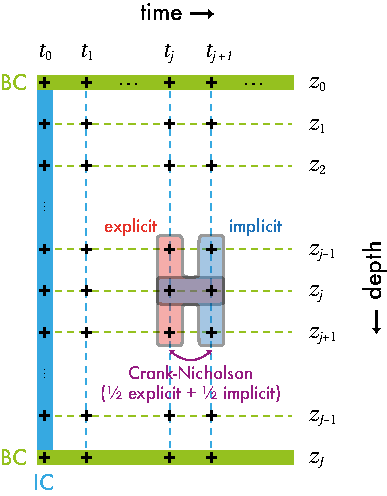
\includegraphics[]{numerical/figures/ztnodes.pdf}
    \caption{A discretization in space and time. Solving a PDE dependent on time and can be done either solving for the future (explicit), 'solving' for the past (implicit), or a mix of both (Crank-Nicholson).}
    \label{fig:ztnodes}
\end{figure}

Finite difference approximations in time mirror those used in space. A forward difference in time estimates the time derivative using information from the present state, while a backward difference estimates it using information from the future state. As in space, the choice of approximation has important implications for accuracy and stability.

\subsection{Physical meaning of time stepping}

Time stepping controls the rate at which information can propagate through the numerical model. For diffusive processes such as heat transport, information propagates through local interactions between neighboring nodes. In a single timestep, changes at a node can influence only adjacent nodes.

If the timestep is chosen too large, the numerical scheme attempts to transmit information faster than the underlying physics allows. In effect, the model is asked to move heat farther in one timestep than diffusion permits---it's like exceeding the speed of light...it can't be done. When this happens, the solution becomes unstable and nonphysical.

This limitation is not merely numerical; it reflects the physics of diffusion.  Numerical schemes must respect the finite rate at which diffusive processes redistribute heat.

\subsection{Explicit (forward-in-time) method}

Consider the one-dimensional heat diffusion equation with constant properties,
\[
    \pdv{T}{t} = \kappa \pdv[2]{T}{z}.
\]
Since many geologists and geochemists encounter diffusion outside of geophysics, it is worth noting that chemical diffusion follows an identical mathematical form. Replacing temperature $T$ with concentration $C$ and thermal diffusivity $\kappa$ with chemical diffusivity $D$ yields the corresponding equation for chemical transport.

Using a forward difference in time and a second-order central difference in space, the finite difference approximation at depth $z_j$ and time $t^{n+1}$ is
\[
    \workeq
    \frac{T_j^{n+1} - T_j^n}{\Delta t} =
    \kappa \frac{T_{j+1}^n - 2T_j^n + T_{j-1}^n}{\Delta z^2}.
\]
Solving for the future temperature gives
\[
    \workeq
    T_j^{n+1} = T_j^n +
    \kappa \frac{\Delta t}{\Delta z^2} \left(T_{j+1}^n - 2T_j^n + T_{j-1}^n\right).
\]

This explicit scheme predicts the future state entirely from the present. It is computationally efficient and straightforward to implement, but it is only stable if the timestep is sufficiently small. Because information propagates only between neighboring nodes in a single timestep, the timestep must satisfy the stability condition
\[
    \coreeq
    \kappa \frac{\Delta t}{\Delta z^2} \le \frac{1}{2}.
\]
If this inequality is violated, numerical errors grow rapidly and the solution becomes unstable. Higher-order spatial discretizations alter the stability criterion but do not remove the fundamental restriction on timestep size.

\subsection{Implicit (backward-in-time) method}

An alternative approach is to evaluate spatial derivatives at the future time level. Using a backward difference in time gives
\[
    \workeq
    \frac{T_j^{n+1} - T_j^n}{\Delta t} =
    \kappa \frac{T_{j+1}^{n+1} - 2T_j^{n+1} + T_{j-1}^{n+1}}{\Delta z^2}.
\]

Rearranging terms places all unknown future temperatures on one side,
\[
    \workeq
    -\kappa \frac{\Delta t}{\Delta z^2} T_{j-1}^{n+1} +
    \left(1 + 2\kappa \frac{\Delta t}{\Delta z^2}\right) T_j^{n+1} -
    \kappa \frac{\Delta t}{\Delta z^2} T_{j+1}^{n+1} =
    T_j^n .
\]

For a domain with fixed temperatures at its boundaries (Dirichlet boundary conditions), the full system of equations can be written explicitly as
\begin{align*}
    T_0^{n+1} &= T_0^{n}, \\
    -\alpha T_{0}^{n+1} + (1 + 2\alpha) T_1^{n+1} - \alpha T_{2}^{n+1} &= T_1^n, \\
    -\alpha T_{1}^{n+1} + (1 + 2\alpha) T_2^{n+1} - \alpha T_{3}^{n+1} &= T_2^n, \\
    &\vdots \\
    -\alpha T_{J-2}^{n+1} + (1 + 2\alpha) T_{J-1}^{n+1} - \alpha T_{J}^{n+1} &= T_{J-1}^n, \\
    T_J^{n+1} &= T_J^{n},
\end{align*}
where $\alpha = \kappa \Delta t / \Delta z^2$.  While this looks like we are using the future to solve for the past, we really don't know the future temperatures and need to solve for it by solving this system of equations.  Because this is a system of linear equations it is easy to write the above result in matrix form:
\begin{align*}
    \begin{bmatrix}
        1 & 0 & 0 & 0 & \cdots & 0 & 0 & 0 & 0 \\
        -\alpha & (1 + 2\alpha) & -\alpha & 0 & \cdots & 0 & 0 & 0 & 0 \\
        0 & -\alpha & (1 + 2\alpha) & -\alpha & \cdots & 0 & 0 & 0 & 0 \\
        \vdots & \ddots & \ddots & \ddots & & & & \vdots \\
        0 & 0 & 0 & 0 & \cdots & -\alpha & (1 + 2\alpha) & -\alpha & 0 \\
        0 & 0 & 0 & 0 & \cdots & 0 & -\alpha & (1 + 2\alpha) & -\alpha \\
        0 & 0 & 0 & 0 & \cdots & 0 & 0 & 0 & 1
    \end{bmatrix}
    \begin{bmatrix}
        T_{0}^{n+1} \\
        T_{1}^{n+1} \\
        T_{2}^{n+1} \\
        \vdots \\
        T_{J-2}^{n+1} \\
        T_{J-1}^{n+1} \\
        T_{J}^{n+1}
    \end{bmatrix}
    = \begin{bmatrix}
        T_{0}^n \\
        T_{1}^n \\
        T_{2}^n \\
        \vdots \\
        T_{J-2}^n \\
        T_{J-1}^n \\
        T_{J}^n
    \end{bmatrix}.
\end{align*}
Note that the matrix is sparse except for values along the diagonal and just above and below.  This is called a tridiagonal matrix.  This system can be written compactly in matrix form as
\[
    \mathbf{A}\,\mathbf{T}^{n+1} = \mathbf{T}^n,
\]
where $\mathbf{A}$ is a tridiagonal matrix. Although it is possible to invert $\mathbf{A}$ directly, this is computationally inefficient. Instead, numerical methods exploit the tridiagonal structure to solve the system rapidly and with minimal memory usage.

The implicit method is unconditionally stable: it remains stable for any choice of $\Delta t$. The cost of this stability is the need to solve a system of equations at each timestep.

\subsection{Crank--Nicolson method}

The Crank--Nicolson method combines the explicit and implicit approaches by averaging the spatial derivative between the current and future time levels,
\[
    \workeq
    \frac{T_j^{n+1} - T_j^n}{\Delta t} = \frac{\kappa}{2}
    \left[
    \frac{T_{j+1}^{n+1} - 2T_j^{n+1} + T_{j-1}^{n+1}}{\Delta z^2} +
    \frac{T_{j+1}^{n} - 2T_j^{n} + T_{j-1}^{n}}{\Delta z^2}
    \right].
\]
As with the implicit scheme, this formulation leads to a tridiagonal system of equations that can be solved efficiently.
Separating the future timestep from the current timestep,
\begin{equation*}
    \workeq
    -\beta T_{j+1}^{n+1} + (1 + 2\beta) T_j^{n+1} - \beta T_{j-1}^{n+1} =
    \beta T_{j+1}^{n} + (1 - 2\beta) T_j^{n} + \beta T_{j-1}^{n} ,
\end{equation*}
where $\beta = \frac{1}{2} \kappa \Delta t \Delta z^{-2}$.  Again we can write this in matrix form producing a tridiagonal matrix,
\begin{align*}
    \resizebox{\textwidth}{!}{$
    \begin{bmatrix}
        1 & 0 & 0 & 0 & \cdots & 0 & 0 & 0 & 0 \\
        -\beta & (1 + 2\beta) & -\beta & 0 & \cdots & 0 & 0 & 0 & 0 \\
        0 & -\beta & (1 + 2\beta) & -\beta & \cdots & 0 & 0 & 0 & 0 \\
        \vdots & \ddots & \ddots & \ddots & & & & \vdots \\
        0 & 0 & 0 & 0 & \cdots & -\beta & (1 + 2\beta) & -\beta & 0 \\
        0 & 0 & 0 & 0 & \cdots & 0 & -\beta & (1 + 2\beta) & -\beta \\
        0 & 0 & 0 & 0 & \cdots & 0 & 0 & 0 & 1
    \end{bmatrix}
    \begin{bmatrix}
        T_{0}^{n+1} \\
        T_{1}^{n+1} \\
        T_{2}^{n+1} \\
        \vdots \\
        T_{J-2}^{n+1} \\
        T_{J-1}^{n+1} \\
        T_{J}^{n+1}
    \end{bmatrix}
    = 
    \begin{bmatrix}
        T_0^n \\
        \beta T_0 + (1 + 2\beta) T_1^n + \beta T_2^n \\
        \beta T_1^n + (1 + 2\beta) T_2^n + \beta T_3^n \\
        \vdots \\
        \beta T_{J-3}^n + (1 + 2\beta) T_{J-2}^n + \beta T_{J-1}^n \\
        \beta T_{J-2}^n + (1 + 2\beta) T_{J-1}^n + \beta T_{J}^n \\
        T_{J}^n
    \end{bmatrix} .
    $}
\end{align*}

The Crank--Nicolson method is second-order accurate in time and stable for linear diffusion problems, providing a balance between numerical accuracy and stability.

\subsection{Depth-dependent sources}

Many geophysical systems include internal sources that vary with depth, such as
radiogenic heat production concentrated in the crust. These sources can be
incorporated naturally into transient diffusion problems.

Including a depth-dependent heat production term $A(z)$, the heat diffusion
equation becomes
\[
    \pdv{T}{t} = \kappa \pdv[2]{T}{z} + \frac{A(z)}{\rho C_P}.
\]
Using a Crank--Nicolson formulation, the finite difference approximation at node $z_j$ is
\[
    \frac{T_j^{n+1} - T_j^n}{\Delta t} =
    \frac{\kappa}{2} \left[
    \frac{T_{j+1}^{n+1} - 2T_j^{n+1} + T_{j-1}^{n+1}}{\Delta z^2} +
    \frac{T_{j+1}^{n} - 2T_j^{n} + T_{j-1}^{n}}{\Delta z^2}
    \right] + \frac{A_j}{\rho C_P} .
\]

The source term appears as an additional contribution to the right-hand side of the system. Importantly, it does not change the coupling between nodes. The resulting system of equations remains tridiagonal and can be solved using the same numerical techniques as in the source-free case.  Depth-dependent sources therefore increase physical realism without altering
the fundamental numerical structure of the problem.

\subsection{Initial conditions}

Time-dependent problems require not only boundary conditions in space, but also an initial condition in time. While boundary conditions constrain how the system interacts with its surroundings, the initial condition specifies the
state of the system at the starting time.  For thermal diffusion problems, the initial condition prescribes the temperature field at time $t = 0$,
\[
    T(z,0) = T_0(z),
\]
or, in discretized form,
\[
    T_j^{0} = T_0(z_j).
\]

The initial condition provides the starting values from which the solution is advanced forward in time. In explicit schemes, these values are used directly to compute the temperature at the next timestep. In implicit and Crank--Nicolson schemes, the initial condition forms the right-hand side of the first system of equations to be solved.  

Initial conditions are not merely mathematical conveniences; they encode physical assumptions about the prior thermal state of the system. Examples include a steady-state geotherm, a uniform initial temperature, or a temperature profile inherited from an earlier tectonic or thermal event.  As with boundary conditions, inappropriate or inconsistent initial conditions can dominate the solution, especially at early times. Careful choice of initial conditions is therefore essential for meaningful transient modeling.

\subsection{Summary of temporal schemes}

Explicit, implicit, and Crank--Nicolson methods differ primarily in how they handle directionality in time. Explicit schemes are forward-looking and computationally inexpensive, but limited by stability constraints. Implicit schemes are backward-looking and stable for any timestep, but require the solution of a linear system. Crank--Nicolson schemes are symmetric in time and offer improved accuracy at the cost of increased computational effort.

As with spatial discretization and boundary conditions, the choice of time stepping scheme reflects a balance between physical realism, numerical stability, and computational efficiency.

\section{PDE Classes}

The numerical behavior of a finite difference model depends strongly on the class of partial differential equation being solved. Although the same basic difference operators appear in many problems, elliptic, parabolic, and hyperbolic equations differ fundamentally in how information propagates through the domain and how solutions must be computed.

The table below summarizes these distinctions using temperature as a unifying example.
\begin{table}
    \centering
    \caption{Common geophysical field equations and their numerical methods.}
    \label{tab:fdpde}
    \begin{tabular}{lcll}
        \toprule
        PDE type & Equation & Information behavior & Numerical consequence \\
        \midrule
        elliptic & $\nabla^2 T = s$ & instantaneous & global solve \\
        parabolic & $\pdv{T}{t} = \kappa\nabla^2T$ & spreads gradually & timestep tied to diffusioin \\
        hyperbolic & $\pdv{T}{t} = c^2\nabla^2T$ & travels at fixed speed & timestep tied to wave speed \\
        \bottomrule
    \end{tabular}
\end{table}

Elliptic equations describe systems in steady state, where changes at one location influence the entire domain instantaneously. Finite difference solutions therefore require solving a global system of equations.

Parabolic equations describe diffusive processes, where information propagates gradually and the system evolves in time. Finite difference solutions advance incrementally, and numerical stability depends on the timestep.

Hyperbolic equations describe wave-like behavior, where information propagates along characteristic paths at finite speed.
The timestep for these problems is limited by how fast information can move through the grid. If the numerical scheme allows a wave to travel farther than one grid cell in a single timestep, the model becomes unstable. In effect, the code is trying to move information faster than the physics allows, and it fails spectacularly.

Finite difference schemes for such equations are constrained by causality and require careful treatment of time stepping and boundary conditions.

\section{Verification}

Numerical solutions should not be accepted on faith. Whenever possible, finite difference models should be tested against analytic solutions or well-known limiting cases. This process, known as verification, ensures that the numerical implementation correctly solves the governing equations.

Common analytic benchmarks for thermal problems include:
\begin{itemize}
  \item steady-state geotherms in homogeneous slabs with prescribed boundary
  temperatures or heat fluxes;
  \item plate cooling or heating of a half-space following a step change
  in boundary temperature.
\end{itemize}

Agreement with analytic solutions builds confidence in the numerical method.  Disagreement usually indicates problems with boundary conditions, grid resolution, timestep choice, or indexing rather than with the physics itself.

Verification should be viewed as an essential part of model development rather than an optional check.

\section{Beyond Linearity}

Most examples in this chapter have assumed constant material properties, planar boundaries, and linear governing equations. These assumptions are useful for developing intuition, but real geologic systems are rarely so simple.  Finite difference methods are flexible enough to accommodate many departures from linearity, provided they are introduced carefully.

Many geophysical problems include sources or sinks that add or remove heat within the domain. Examples include radiogenic heat production, latent heat associated with phase changes, or chemical reactions.  For transient heat diffusion, an internal source term $A(z)$ can be included directly in the governing equation,
\[
    \pdv{T}{t} = \kappa \pdv[2]{T}{z} + \frac{A}{\rho c_p}.
\]
In a finite difference formulation, source terms enter as additional terms in the update equation at each node. Conceptually, they act as local forcing that raises or lowers temperature independent of diffusion.

In many geologic settings, thermal conductivity is directionally dependent.  Layered sediments, foliated metamorphic rocks, and fractured media may conduct heat more efficiently in one direction than another.  Anisotropy is handled naturally in finite difference methods by allowing different conductivities (or diffusivities) in different coordinate directions. In two dimensions, this leads to diffusion terms of the form
\[
\pdv{}{x}\!\left(k_x \pdv{T}{x}\right)
+
\pdv{}{z}\!\left(k_z \pdv{T}{z}\right),
\]
which can be discretized using the same stencil ideas developed earlier, with direction-dependent coefficients.

Thermal conductivity, heat capacity, and diffusivity often vary with temperature. Pressure dependence is commonly incorporated by prescribing depth- dependent properties at the outset of a model, but temperature dependence introduces true nonlinearity.  In finite difference models, temperature-dependent properties are typically handled iteratively. At each timestep, material properties are updated using the current temperature field, and the governing equations are solved again using the updated values. Convergence is assessed by monitoring changes in the solution between iterations.

\subsection{Topography and nonplanar boundaries}

The Earth's surface and many internal boundaries are not flat. Surface topography and basal relief can strongly influence heat flow, especially near the surface.

In finite difference methods, nonplanar boundaries are often handled by:
\begin{itemize}
  \item mapping the physical domain onto a rectangular computational grid;
  \item approximating topography using stair-step boundaries aligned with the grid;
  \item or modifying boundary conditions locally to account for variable surface elevation.
\end{itemize}

While such approaches can be effective, strongly irregular geometries often motivate the use of finite element or finite volume methods, which handle complex boundaries more naturally.

\section{Other Methods}

Finite difference methods are among the simplest and most transparent ways to solve partial differential equations, but they also have important limitations:
\begin{itemize}
    \item Finite difference methods are most naturally formulated on structured (logically rectangular) grids, which can make complex geometries and highly irregular boundaries difficult to represent accurately.
    \item Grid refinement around regions of interest is possible, but often leads to large aspect ratios or strongly varying cell sizes elsewhere in the domain, which can degrade numerical accuracy or impose restrictive timestep constraints.
    \item When material advects through the domain, finite difference models must either track properties moving through a fixed grid or deform the grid itself. Grid deformation can introduce very small cell sizes that require correspondingly small timesteps to maintain stability.
\end{itemize}

Finite differences are therefore not the only option. Two other approaches are widely used in geophysics and engineering: finite element methods and finite volume methods.

Finite element methods (FEM) approximate the solution using basis functions defined over elements that tile the domain. They are particularly well suited to complex geometries, irregular boundaries, and strongly heterogeneous materials.  Finite element meshes can be refined locally around regions of interest and can be deformed more naturally to accommodate material motion and advection.  Compared to finite difference methods, FEM formulations are mathematically and computationally more complex, but offer greater geometric flexibility.

Finite volume methods (FVM) enforce conservation laws by integrating governing equations over control volumes. Fluxes are computed explicitly across volume boundaries, making these methods especially effective for problems where strict conservation is critical, such as fluid flow, mass transport, and reactive systems. In some formulations, control volumes can move with the material, providing a natural framework for advection while preserving conservation.

Compared to finite differences:
\begin{itemize}
  \item finite difference methods are conceptually simpler and easier to implement;
  \item finite element methods handle complex geometries and boundary conditions more naturally;
  \item finite volume methods emphasize conservation and robustness, particularly in advective systems.
\end{itemize}

\section{Looking Ahead}

In this course, we have focused on finite difference methods because they provide a direct and transparent connection between physical laws and their numerical implementation. This clarity makes finite differences especially well suited for developing intuition about how geophysical systems behave and how numerical models encode physical assumptions. Finite element and finite volume methods are typically introduced in more advanced numerical modeling courses, where their additional mathematical and computational complexity can be addressed in greater depth.

The techniques developed in this chapter form the foundation for modeling many realistic geophysical systems. Incorporating nonlinearity, anisotropy, sharp property contrasts, and complex boundaries increases physical realism, but also demands greater care in assessing stability, convergence, and physical interpretation. These challenges motivate more sophisticated discretization strategies and solution methods, some of which were briefly introduced here and are treated more fully in advanced courses.

Numerical forward models such as those developed in this chapter are also a central component of inversion theory. Inverse problems seek to infer subsurface properties or boundary conditions from observations by repeatedly evaluating forward models and comparing their predictions to data. The accuracy, stability, and efficiency of finite difference solutions therefore play a key role in determining what information can be reliably extracted from geophysical measurements. The next chapter builds on the numerical foundations developed here to introduce the principles of inversion and data interpretation.
